% tracking_efficiency_matching.tex
% Simple TikZ figure explaining how hit-matching (tracking) efficiency is
% computed in the MALTA simulation analysis chain (analysis_multiPlane).
% Compile:  pdflatex tracking_efficiency_matching.tex

\documentclass[tikz]{standalone}
\usepackage{tikz}
\usepackage{amsmath}
\usetikzlibrary{arrows.meta, calc, decorations.pathreplacing}

\begin{document}
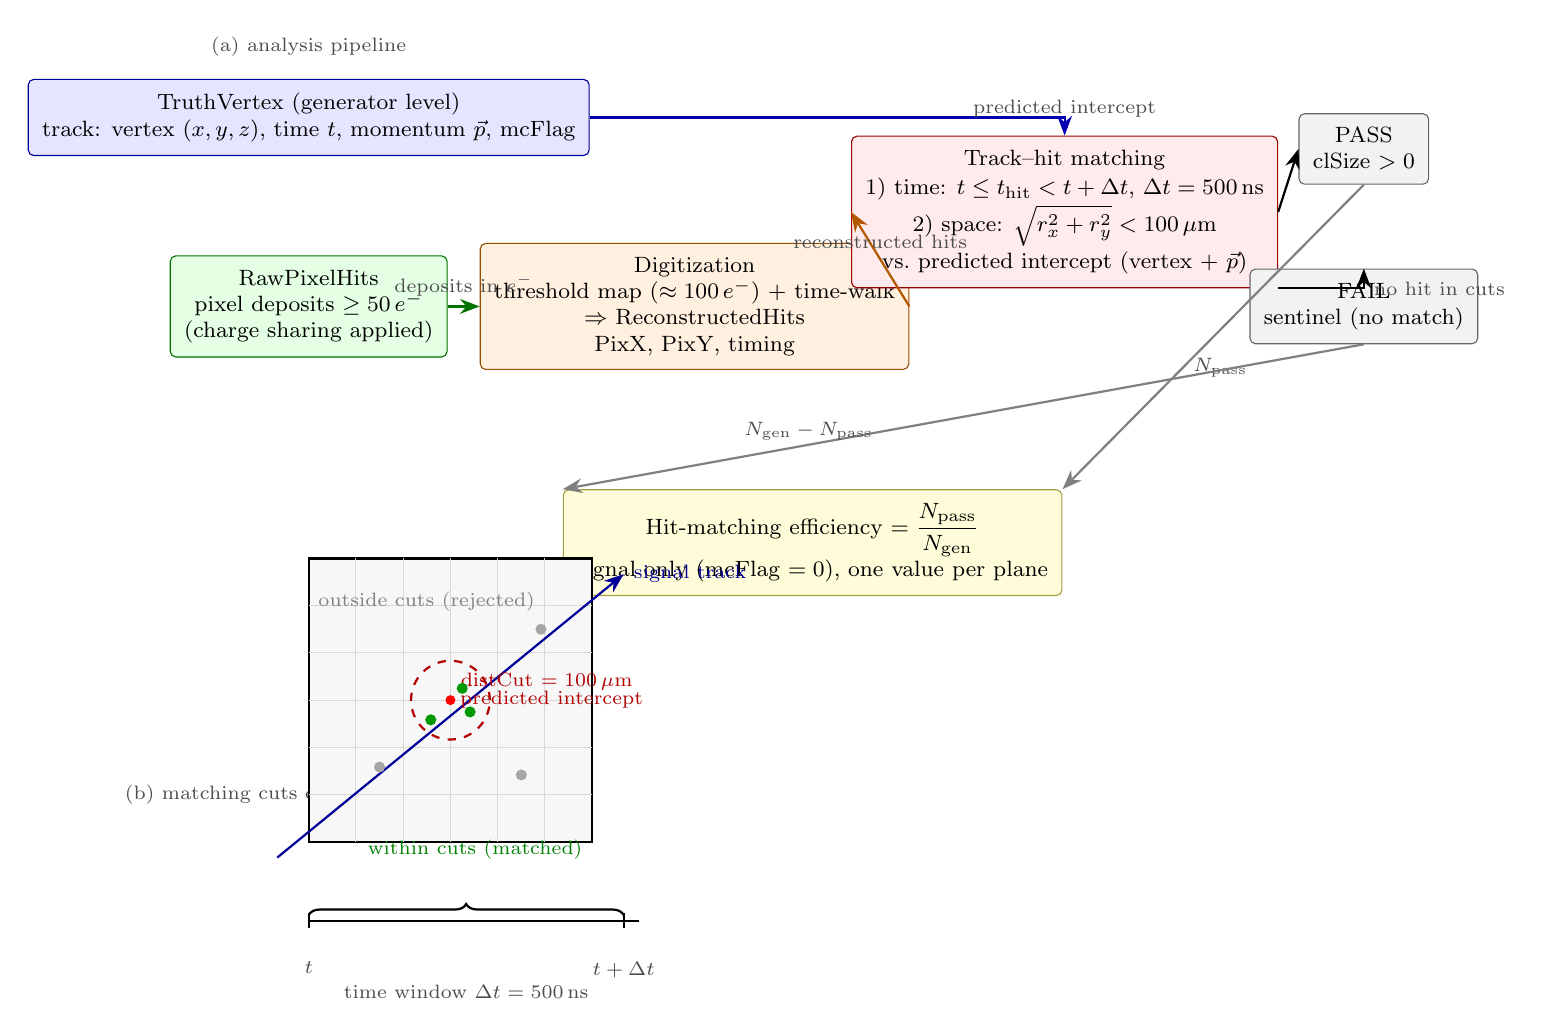
\begin{tikzpicture}[
  font=\footnotesize,
  box/.style={draw, rounded corners=2pt, align=center, inner sep=5pt},
  truth/.style={box, fill=blue!10,   draw=blue!60!black},
  rawst/.style={box, fill=green!10,  draw=green!45!black},
  digit/.style={box, fill=orange!12, draw=orange!60!black},
  matchbox/.style={box, fill=red!8,  draw=red!60!black},
  outbox/.style={box, fill=gray!10,  draw=black!60},
  effbox/.style={box, fill=yellow!15, draw=yellow!60!black},
  arr/.style={-{Stealth[length=2.5mm]}, thick},
  lab/.style={font=\scriptsize, text=black!70},
]

% ---------------------------------------------------------------
% (a) Analysis pipeline
% ---------------------------------------------------------------
\node[lab] at (0,0.9) {(a) analysis pipeline};

\node[truth] (tr) at (0,0) {TruthVertex (generator level)\\track: vertex $(x,y,z)$, time $t$, momentum $\vec{p}$, mcFlag};
\node[rawst] (raw) at (0,-2.4) {RawPixelHits\\pixel deposits $\ge 50\,e^{-}$\\(charge sharing applied)};
\node[digit] (dig) at (4.9,-2.4) {Digitization\\threshold map ($\approx 100\,e^{-}$) + time-walk\\$\Rightarrow$ ReconstructedHits\\PixX, PixY, timing};
\node[matchbox] (mt) at (9.6,-1.2) {Track--hit matching\\[1pt]
                                1) time: $t \le t_{\rm hit} < t + \Delta t$, $\Delta t = 500$\,ns\\[1pt]
                                2) space: $\sqrt{r_x^{2}+r_y^{2}} < 100\,\mu$m\\[1pt]
                                vs.\ predicted intercept (vertex + $\vec{p}$)};
\node[outbox] (pass) at (13.4,-0.4) {PASS\\clSize $> 0$};
\node[outbox] (fail) at (13.4,-2.4) {FAIL\\sentinel (no match)};
\node[effbox] (eff) at (6.4,-5.4) {Hit-matching efficiency $= \dfrac{N_{\rm pass}}{N_{\rm gen}}$\\signal only (mcFlag $=0$), one value per plane};

\draw[arr, blue!70!black] (tr.east) -| (mt.north) node[pos=0.78, lab, above]{predicted intercept};
\draw[arr, green!45!black] (raw.east) -- (dig.west) node[midway, lab, above]{deposits in $e^{-}$};
\draw[arr, orange!70!black] (dig.east) -- (mt.west) node[midway, lab, above]{reconstructed hits};
\draw[arr] (mt.east) -- (pass.west);
\draw[arr] (mt.south east) -| (fail.north) node[pos=0.5, lab, right]{no hit in cuts};
\draw[arr, gray] (pass.south) -- (eff.north east) node[pos=0.6, lab, right]{$N_{\rm pass}$};
\draw[arr, gray] (fail.south) -- (eff.north west) node[pos=0.6, lab, left]{$N_{\rm gen}-N_{\rm pass}$};

% ---------------------------------------------------------------
% (b) Matching cuts on one sensor plane
% ---------------------------------------------------------------
\begin{scope}[shift={(0,-9.2)}]
  \node[lab] at (0,0.6) {(b) matching cuts on the sensor plane};

  % sensor with faint pixel grid
  \fill[black!3] (0,0) rectangle (3.6,3.6);
  \draw[thick] (0,0) rectangle (3.6,3.6);
  \foreach \i in {1,...,5} {
    \draw[black!15] (\i*0.6,0) -- (\i*0.6,3.6);
    \draw[black!15] (0,\i*0.6) -- (3.6,\i*0.6);
  }

  % particle track crossing the plane
  \draw[arr, blue!60!black] (-0.4,-0.2) -- (4.0,3.4) node[right, lab, blue!60!black]{signal track};
  \fill[red] (1.8,1.8) circle (1.8pt) node[right, lab, red!70!black]{predicted intercept};
  \draw[red!70!black, dashed, thick] (1.8,1.8) circle (0.5) node[above right, lab, red!70!black]{distCut $=100\,\mu$m};

  % hits inside the cut (matched) and outside (rejected)
  \fill[green!60!black] (1.95,1.95) circle (2pt);
  \fill[green!60!black] (1.55,1.55) circle (2pt);
  \fill[green!60!black] (2.05,1.65) circle (2pt);
  \fill[gray!70] (2.95,2.7) circle (2pt);
  \fill[gray!70] (0.9,0.95) circle (2pt);
  \fill[gray!70] (2.7,0.85) circle (2pt);
  \node[lab, green!50!black] at (3.6,0.15) [anchor=north east]{within cuts (matched)};
  \node[lab, gray] at (0,3.3) [anchor=north west]{outside cuts (rejected)};

  % time-window bar
  \draw[thick] (0,-1.0) -- (4.2,-1.0);
  \draw[thick] (0,-1.1) -- (0,-0.9);
  \draw[thick] (4.0,-1.1) -- (4.0,-0.9);
  \node[lab] at (0,-1.4) [anchor=north]{$t$};
  \node[lab] at (4.0,-1.4) [anchor=north]{$t + \Delta t$};
  \draw[decorate, decoration={brace, amplitude=4pt, raise=2pt}, thick] (0,-1.0) -- (4.0,-1.0);
  \node[lab] at (2.0,-1.9) {time window $\Delta t = 500$\,ns};
\end{scope}

\end{tikzpicture}
\end{document}
